\documentclass{beamer}

\usepackage{graphicx}
\usepackage[utf8]{inputenc}
\usepackage[T1]{fontenc}
\usepackage{lmodern}
\usepackage[english]{babel}
\usepackage{amsmath}
\usepackage{amsthm}
\usepackage{mathtools}
\usepackage{amssymb}
\usepackage{listings}
\usepackage{xparse}
\usepackage{stmaryrd}
\usepackage{geometry}
\usepackage{enumerate}
\usepackage{hyperref}
\usepackage{tikz}
\usepackage{pgfplots}
\usepackage{stmaryrd}
\usepackage[style=english]{csquotes}
\usepackage[language=english, backend=biber, style=alphabetic, sorting=nyt]{biblatex}

\hypersetup{
    colorlinks,
    linkcolor={red!50!black},
    citecolor={blue!50!black},
    urlcolor={blue!80!black}
}

\usetikzlibrary{babel, positioning, shapes.geometric, arrows, arrows.meta}
\addbibresource{../../bibliography.bib}

\title{FHE Reading Group - January 20\\Linear Transform in in BFV (Bootstrapping)}
\author{Simon Pohmann}

\newcommand{\Z}{\mathbb{Z}}
\newcommand{\F}{\mathbb{F}}
\newcommand{\C}{\mathbb{C}}
\newcommand{\I}{\mathbb{I}}
\newcommand{\V}{\mathbb{V}}
\newcommand{\End}{\mathrm{End}}
\newcommand{\Quot}{\mathrm{Quot}}
\newcommand{\Half}{\mathcal{H}}
\newcommand{\Lattice}{\mathcal{L}}
\newcommand{\divides}{\ \mid \ }
\newcommand{\notdivides}{\ \nmid \ }
\newcommand{\Cl}{\mathrm{Cl}}
\newcommand{\K}{\mathcal{K}}
\newcommand{\p}{\mathfrak{p}}
\newcommand{\q}{\mathfrak{q}}
\newcommand{\val}{v}
\renewcommand{\l}{\mathfrak{l}}
\renewcommand{\a}{\mathfrak{a}}
\renewcommand{\b}{\mathfrak{b}}
\renewcommand{\O}{\mathcal{O}}

\newcommand\restr[2]{{
    \left.\kern-\nulldelimiterspace
    #1
    \vphantom{\big|}
    \right|_{#2}
}}

\newtheorem{remark}{Remark}
\newtheorem{prop}{Proposition}
\newtheorem{heuristic}{Heuristic}

\begin{document}

\begin{frame}
    \maketitle
\end{frame}

\begin{frame}
    \frametitle{Where do we use it?}

    \begin{center}
        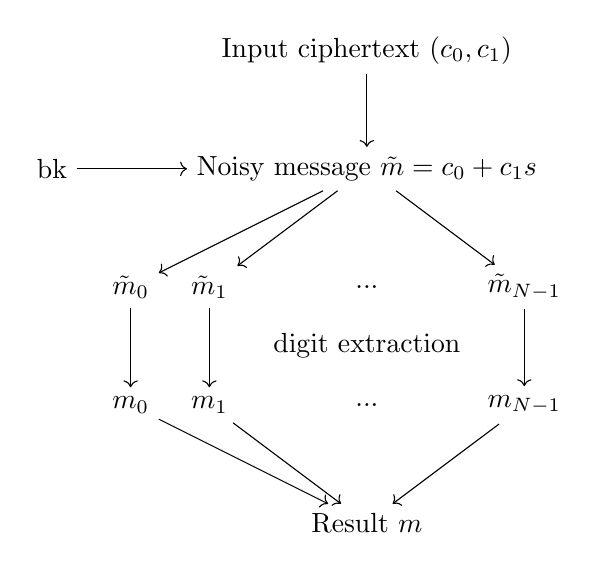
\begin{tikzpicture}
            \node (input) at (0, 0) {Input ciphertext $(c_0, c_1)$};
            \node (bk) at (-4, -1.5) {$\mathrm{bk}$};
            \node (noisy_message) at (0, -1.5) {Noisy message $\tilde{m} = c_0 + c_1 s$};
            \node (coeff1) at (-3, -3) {$\tilde{m}_0$};
            \node (coeff2) at (-2, -3) {$\tilde{m}_1$};
            \node (coeff) at (0, -3) {$...$};
            \node (coeffn) at (2, -3) {$\tilde{m}_{N - 1}$};
            \node (rcoeff1) at (-3, -4.5) {$m_0$};
            \node (rcoeff2) at (-2, -4.5) {$m_1$};
            \node (rcoeff) at (0, -4.5) {$...$};
            \node (rcoeffn) at (2, -4.5) {$m_{N - 1}$};
            \node at (0, -3.75) {digit extraction};
            \node (result) at (0, -6) {Result $m$};

            \draw [->] (input) -- (noisy_message);
            \draw [->] (bk) -- (noisy_message);
            \draw [->] (noisy_message) -- (coeff1);
            \draw [->] (noisy_message) -- (coeff2);
            \draw [->] (noisy_message) -- (coeffn);
            \draw [->] (coeff1) -- (rcoeff1);
            \draw [->] (coeff2) -- (rcoeff2);
            \draw [->] (coeffn) -- (rcoeffn);
            \draw [->] (rcoeff1) -- (result);
            \draw [->] (rcoeff2) -- (result);
            \draw [->] (rcoeffn) -- (result);
        \end{tikzpicture}
    \end{center}
\end{frame}

\begin{frame}
    \frametitle{SIMD via slots}

    Plaintext space is $\mathcal{P} = R/p^eR$, where $R = \Z[X]/(X^N + 1)$; Assume $e = 1$
    \\$\quad \Rightarrow$ $\mathcal{P} = \F_p[X]/(X^N + 1)$
    \begin{remark}
        $X^N + 1$ is irreducible in $\Z$
    \end{remark}
    \begin{prop}
        \begin{itemize}
            \item $X^N + 1 \equiv f_1 ... f_n \mod p$ where $n = \mathrm{ord}_{(\Z/2N\Z)^*}(p)$
            \item $f_i$ irreducible of degree $d = N/n$
        \end{itemize}
    \end{prop}
    \begin{equation*}
        \Rightarrow \quad \mathcal{P} \cong \bigoplus_{i = 1}^n \F_{p^d}
    \end{equation*}
    One operation in $\mathcal{P}$ $\approx$ $n$ operations, one on each slot $\F_{p^d}$
\end{frame}

\begin{frame}
    \frametitle{Using it}

    \begin{center}
        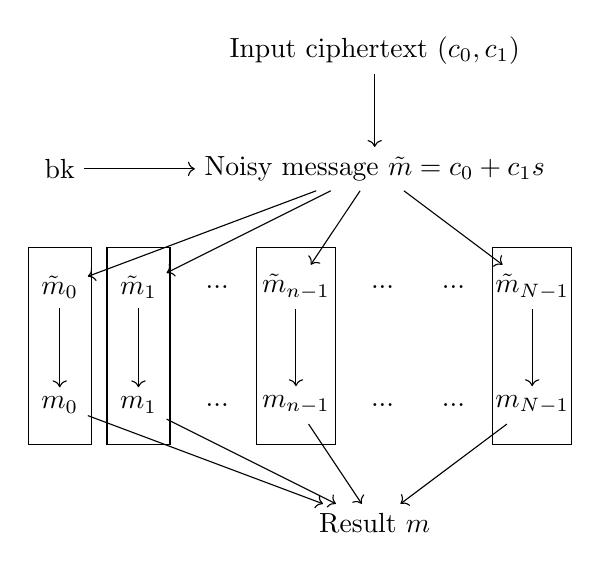
\begin{tikzpicture}
            \node (input) at (0, 0) {Input ciphertext $(c_0, c_1)$};
            \node (bk) at (-4, -1.5) {$\mathrm{bk}$};
            \node (noisy_message) at (0, -1.5) {Noisy message $\tilde{m} = c_0 + c_1 s$};
            \node (coeff1) at (-4, -3) {$\tilde{m}_0$};
            \node (coeff2) at (-3, -3) {$\tilde{m}_1$};
            \node (coeff3) at (-1, -3) {$\tilde{m}_{n - 1}$};
            \node at (-2, -3) {$...$};
            \node at (0.1, -3) {$...$};
            \node at (1, -3) {$...$};
            \node (coeffn) at (2, -3) {$\tilde{m}_{N - 1}$};
            \node (rcoeff1) at (-4, -4.5) {$m_0$};
            \node (rcoeff2) at (-3, -4.5) {$m_1$};
            \node (rcoeff3) at (-1, -4.5) {$m_{n - 1}$};
            \node at (-2, -4.5) {$...$};
            \node at (0.1, -4.5) {$...$};
            \node at (1, -4.5) {$...$};
            \node (rcoeffn) at (2, -4.5) {$m_{N - 1}$};
            \node (result) at (0, -6) {Result $m$};

            \draw [->] (input) -- (noisy_message);
            \draw [->] (bk) -- (noisy_message);
            \draw [->] (noisy_message) -- (coeff1);
            \draw [->] (noisy_message) -- (coeff2);
            \draw [->] (noisy_message) -- (coeff3);
            \draw [->] (noisy_message) -- (coeffn);
            \draw [->] (coeff1) -- (rcoeff1);
            \draw [->] (coeff2) -- (rcoeff2);
            \draw [->] (coeff3) -- (rcoeff3);
            \draw [->] (coeffn) -- (rcoeffn);
            \draw [->] (rcoeff1) -- (result);
            \draw [->] (rcoeff2) -- (result);
            \draw [->] (rcoeff3) -- (result);
            \draw [->] (rcoeffn) -- (result);

            \draw[draw=black] (-4.4, -2.5) rectangle (-3.6, -5);
            \draw[draw=black] (-3.4, -2.5) rectangle (-2.6, -5);
            \draw[draw=black] (-1.5, -2.5) rectangle (-0.5, -5);
            \draw[draw=black] (1.5, -2.5) rectangle (2.5, -5);
        \end{tikzpicture}
    \end{center}
    $N$ digit extractions
\end{frame}

\begin{frame}
    \frametitle{Using it (cont'd)}

    \begin{center}
        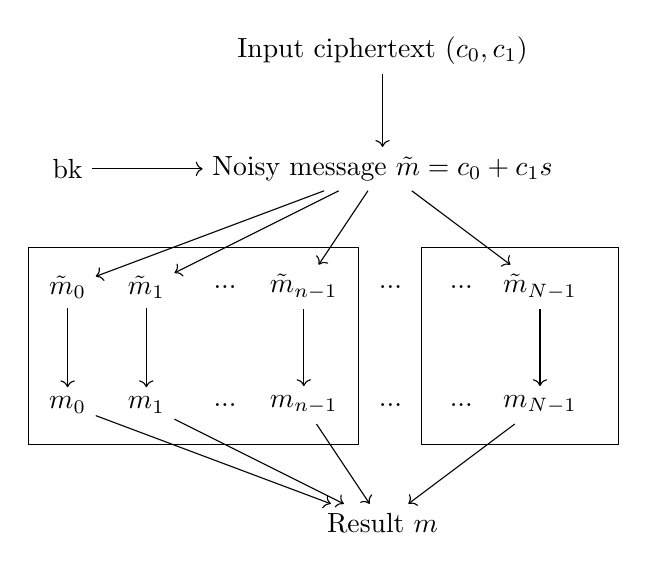
\begin{tikzpicture}
            \node (input) at (0, 0) {Input ciphertext $(c_0, c_1)$};
            \node (bk) at (-4, -1.5) {$\mathrm{bk}$};
            \node (noisy_message) at (0, -1.5) {Noisy message $\tilde{m} = c_0 + c_1 s$};
            \node (coeff1) at (-4, -3) {$\tilde{m}_0$};
            \node (coeff2) at (-3, -3) {$\tilde{m}_1$};
            \node (coeff3) at (-1, -3) {$\tilde{m}_{n - 1}$};
            \node at (-2, -3) {$...$};
            \node at (0.1, -3) {$...$};
            \node at (1, -3) {$...$};
            \node (coeffn) at (2, -3) {$\tilde{m}_{N - 1}$};
            \node (rcoeff1) at (-4, -4.5) {$m_0$};
            \node (rcoeff2) at (-3, -4.5) {$m_1$};
            \node (rcoeff3) at (-1, -4.5) {$m_{n - 1}$};
            \node at (-2, -4.5) {$...$};
            \node at (0.1, -4.5) {$...$};
            \node at (1, -4.5) {$...$};
            \node (rcoeffn) at (2, -4.5) {$m_{N - 1}$};
            \node (result) at (0, -6) {Result $m$};

            \draw [->] (input) -- (noisy_message);
            \draw [->] (bk) -- (noisy_message);
            \draw [->] (noisy_message) -- (coeff1);
            \draw [->] (noisy_message) -- (coeff2);
            \draw [->] (noisy_message) -- (coeff3);
            \draw [->] (noisy_message) -- (coeffn);
            \draw [->] (coeff1) -- (rcoeff1);
            \draw [->] (coeff2) -- (rcoeff2);
            \draw [->] (coeff3) -- (rcoeff3);
            \draw [->] (coeffn) -- (rcoeffn);
            \draw [->] (rcoeff1) -- (result);
            \draw [->] (rcoeff2) -- (result);
            \draw [->] (rcoeff3) -- (result);
            \draw [->] (rcoeffn) -- (result);

            \draw[draw=black] (-4.5, -2.5) rectangle (-0.3, -5);
            \draw[draw=black] (0.5, -2.5) rectangle (3, -5);
        \end{tikzpicture}
    \end{center}
    $N/n$ digit extractions
\end{frame}

\begin{frame}
    \frametitle{Using it (cont'd)}

    \begin{center}
        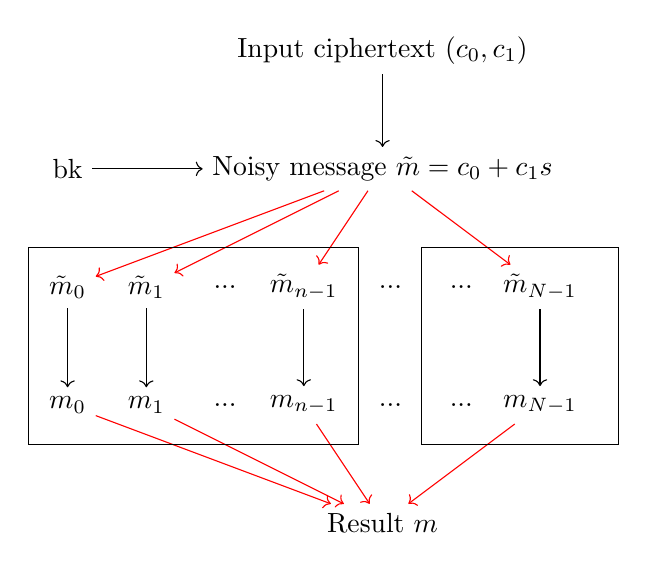
\begin{tikzpicture}
            \node (input) at (0, 0) {Input ciphertext $(c_0, c_1)$};
            \node (bk) at (-4, -1.5) {$\mathrm{bk}$};
            \node (noisy_message) at (0, -1.5) {Noisy message $\tilde{m} = c_0 + c_1 s$};
            \node (coeff1) at (-4, -3) {$\tilde{m}_0$};
            \node (coeff2) at (-3, -3) {$\tilde{m}_1$};
            \node (coeff3) at (-1, -3) {$\tilde{m}_{n - 1}$};
            \node at (-2, -3) {$...$};
            \node at (0.1, -3) {$...$};
            \node at (1, -3) {$...$};
            \node (coeffn) at (2, -3) {$\tilde{m}_{N - 1}$};
            \node (rcoeff1) at (-4, -4.5) {$m_0$};
            \node (rcoeff2) at (-3, -4.5) {$m_1$};
            \node (rcoeff3) at (-1, -4.5) {$m_{n - 1}$};
            \node at (-2, -4.5) {$...$};
            \node at (0.1, -4.5) {$...$};
            \node at (1, -4.5) {$...$};
            \node (rcoeffn) at (2, -4.5) {$m_{N - 1}$};
            \node (result) at (0, -6) {Result $m$};

            \draw [->] (input) -- (noisy_message);
            \draw [->] (bk) -- (noisy_message);
            \draw [->, red] (noisy_message) -- (coeff1);
            \draw [->, red] (noisy_message) -- (coeff2);
            \draw [->, red] (noisy_message) -- (coeff3);
            \draw [->, red] (noisy_message) -- (coeffn);
            \draw [->] (coeff1) -- (rcoeff1);
            \draw [->] (coeff2) -- (rcoeff2);
            \draw [->] (coeff3) -- (rcoeff3);
            \draw [->] (coeffn) -- (rcoeffn);
            \draw [->, red] (rcoeff1) -- (result);
            \draw [->, red] (rcoeff2) -- (result);
            \draw [->, red] (rcoeff3) -- (result);
            \draw [->, red] (rcoeffn) -- (result);

            \draw[draw=black] (-4.5, -2.5) rectangle (-0.3, -5);
            \draw[draw=black] (0.5, -2.5) rectangle (3, -5);
        \end{tikzpicture}
    \end{center}
    \begin{center}
        \textcolor{red}{``Evaluation map''}
    \end{center}
\end{frame}

\begin{frame}
    \frametitle{The ``Evaluation map''}
    \begin{align*}
        \text{``Evaluation map''}: \quad \mathcal{P} \ &\to \ \bigoplus \F_{p^d} \cong \mathcal{P} \\ 
        \sum a_i X^i \ &\mapsto \ (a_i)_{0 \leq i < d}
    \end{align*}
    It is $\F_p$-linear!
    \begin{prop}
        The $\F_p$-vector space
        \begin{equation*}
            \mathcal{L} := \{ f: \mathcal{P} \to \mathcal{P} \ | \ \text{$f$ $\F_p$-linear}\}
        \end{equation*}
        is spanned by
        \begin{align*}
            &\{ m_k: \alpha \mapsto X^k \alpha \ | \ k \in \{ 0, ..., N - 1\} \} \\
            &\circ \ \{ \sigma_k: X \mapsto X^k \ | \ k \in (\Z/2N\Z)^* \}
        \end{align*}
    \end{prop}
\end{frame}

\begin{frame}
    \frametitle{Computing linear transforms}
    
    \begin{prop}
        The $\F_p$-vector space
        \begin{equation*}
            \mathcal{L} := \{ f: \mathcal{P} \to \mathcal{P} \ | \ \text{$f$ $\F_p$-linear}\}
        \end{equation*}
        is spanned by
        \begin{align*}
            &\{ m_k: \alpha \mapsto X^k \alpha \ | \ k \in \{ 0, ..., N - 1\} \} \\
            &\circ \ \{ \sigma_k: X \mapsto X^k \ | \ k \in (\Z/2N\Z)^* \}
        \end{align*}
    \end{prop}
    $\Rightarrow$ Every $\F_p$-linear map can be written as
    \begin{equation*}
        \alpha \mapsto \sum_{k \in (\Z/2N\Z)^*} a_k \sigma_k(\alpha)
    \end{equation*}
    where $a_k \in \mathcal{P}$
\end{frame}

\begin{frame}
    \frametitle{More intuitive structure - or how to find the $a_k$}
    \begin{itemize}
        \item $k \in \langle p \rangle \subseteq (\Z/2N\Z)^*$ $\Rightarrow$ $\sigma_k$ is Frobenius within each slot
        \item Otherwise $\Rightarrow$ $\sigma_k$ permutes slots (up to inter-slot auto.)
    \end{itemize}
    We have
    \begin{equation*}
        (\Z/2N\Z)^*/\langle p \rangle = \langle g_1 \rangle \times ... \times \langle g_r \rangle
    \end{equation*}
    $\Rightarrow$ $(\Z/2N\Z)^*/\langle p \rangle$ has structure of an $r$-dimensional hypercube
    \\~\\
    \textbf{We fix a ``slot 0''} (arbitrarily) $\Rightarrow$ Slots inherit hypercube structure
    \begin{equation*}
        S: \mathcal{P} \ \overset{\sim}{\longrightarrow} \ \bigoplus_{I \in (\Z/2N\Z)^*/\langle p \rangle} \F_{p^d}
    \end{equation*}
\end{frame}

\begin{frame}
    \frametitle{More intuitive structure - or how to find the $a_k$ (cont'd)}

    \textbf{Example}: $r = 3$, $(\mathrm{ord}(g_1), \mathrm{ord}(g_2), \mathrm{ord}(g_3)) = (7, 4, 2)$
    \begin{center}
        \includegraphics{hypercube.pdf}
    \end{center}
\end{frame}

\begin{frame}
    \frametitle{Good and bad dimensions}

    \textbf{Problem}: $k \notin \langle p \rangle$ $\Rightarrow$ $\sigma_k$ permutes slots \textcolor{red}{\textbf{(up to inter-slot auto.)}}
    \begin{center}
        Slots have no ``natural'' generator / $\F_{p^d}$ unique only up to iso. - what do we mean by inter-slot automorphism?
    \end{center}
    \begin{center}
        \includegraphics{interslot_auto.pdf}
    \end{center}
\end{frame}

\begin{frame}
    \frametitle{Good and bad dimensions (cont'd)}

    We require that $\sigma_{g_i^{d_i}}$ is identity ($d_i$ hypercube length)
    \begin{prop}
        $\sigma_{g_i^{d_i}} = \mathrm{id} \quad \Leftrightarrow \quad \mathrm{ord}_{(\Z/2N\Z)^*}(g_i) = d_i$.
        \\(note that $d_i = \mathrm{ord}_{(\Z/2N\Z)^*/\langle p \rangle}$)
    \end{prop}
    \begin{itemize}
        \item If this is the case, we call the $i$-th dimension \emph{good}
        \item Otherwise, we call it \emph{bad}
    \end{itemize}
    \begin{remark}
        If $i$-th dim is bad, we can still compute the rotation as
        \begin{equation*}
            \alpha \mapsto \sigma_{g_1^\delta}(\alpha \cdot e) + \sigma_{g_1^{D - \delta}}(\alpha \cdot (1 - e))
        \end{equation*}
        where
        \begin{equation*}
            D = \mathrm{ord}_{(\Z/2N\Z)^*}(g_1)
        \end{equation*}
        and $e$ is 1 in the first $d_i - \delta$ slots, and $0$ in the others
    \end{remark}
\end{frame}

\begin{frame}
    \frametitle{Good and bad dimensions (cont'd)}

    \begin{itemize}
        \item Some dimensions are good, some bad
        \item Rotation in good dimension: 1 Galois op
        \item Rotation in bad dimension: 2 Galois ops
    \end{itemize}
    \begin{prop}
        We can choose the $g_i$ such that only one dimension is bad
    \end{prop}
    ~\\
    \textbf{So far}: Rotations along a hypercube axis are easier to understand than the action of the group $(\Z/2N\Z)^*$ via $\sigma_{\cdot}$
\end{frame}

\begin{frame}
    \frametitle{Back to the evaluation map}

    We want to write the evaluation map as a linear transform
    \\~\\
    We explain the map
    \begin{equation*}
        \mathrm{Eval}: \mathcal{P} \cong \bigoplus \F_{p^d} \to \mathcal{P}, \quad (a_i) \mapsto \sum a_i X^i
    \end{equation*}
    \begin{remark}
        There are ``intermediate representations'' in the decomposition
        \begin{equation*}
            \mathcal{P} \cong \bigoplus^{d_1} \bigoplus^{d_2} ... \bigoplus^{d_r} \F_{p^d}
        \end{equation*}
        Let
        \begin{equation*}
            \mathcal{P}_i = \bigoplus^{d_i} ... \bigoplus^{d_r} \F_{p^d} \quad \Rightarrow \quad \mathcal{P} = \bigoplus^{d_1} ... \bigoplus^{d_{i - 1}} \mathcal{P}_i
        \end{equation*}
    \end{remark} 
\end{frame}

\begin{frame}
    \frametitle{Back to the evaluation map (cont'd)}

    \begin{equation*}
        \mathrm{Eval}: \mathcal{P} \cong \bigoplus \F_{p^d} \to \mathcal{P}, \quad (a_i) \mapsto \sum a_i X^i
    \end{equation*}
    Do $\mathrm{Eval}$ along one hypercube dim:
    \begin{align*}
        \mathrm{Eval}_i: \bigoplus^{d_1} ... \bigoplus^{d_i} \mathcal{P}_{i + 1} \ &\to \ \bigoplus^{d_1} ... \bigoplus^{d_{i - 1}} \mathcal{P}_i \\
        \Bigl( (a_{j_1, ..., j_i})_{j_i} \Bigr)_{j_1, ..., j_{i - 1}} \ &\mapsto \ \Bigl( \sum_{j_i} a_{j_1, ..., j_i} \zeta_i^{j_i} \Bigr)_{j_1, ..., j_{i - 1}}
    \end{align*}
    where $\zeta_i = X^{d_{i + 2} ... d_r}$
    \begin{equation*}
        \Rightarrow \quad \mathrm{Eval} = \mathrm{Eval}_1 \circ ... \circ \mathrm{Eval}_r
    \end{equation*}
\end{frame}

\begin{frame}
    \frametitle{Back to the evaluation map (cont'd)}

    \begin{center}
        \includegraphics{reduce.pdf}
    \end{center}
\end{frame}

\begin{frame}
    \frametitle{Why all of this?}

    We can just solve a (huge) linear system to find $a_k \in \mathcal{P}$ such that
    \begin{equation*}
        \alpha \mapsto \sum_{k \in (\Z/2N\Z)^*} a_k \sigma_k(\alpha)
    \end{equation*}
    is the transform.
    \\~\\
    \textbf{Two Reasons}
    \begin{itemize}
        \item The system is not easy to solve (irrelevant in practice)
        \item Performance!
        \begin{itemize}
            \item In some cases, we can compute $\mathrm{Eval}_i$ with 1 resp. 2 autos.!
            \item Runtime: $2\log_2(n)$ autos. instead of $n$ (or $2\sqrt{n}$)!
            \item Which cases? dimension is good!
        \end{itemize}
    \end{itemize}
\end{frame}

\begin{frame}
    \frametitle{Good dimensions and the factorization of $\mathrm{Eval}$}

    \textbf{Problem}: $k \notin \langle p \rangle$ $\Rightarrow$ $\sigma_k$ permutes slots \textcolor{red}{\textbf{(up to inter-slot auto.)}}
    \begin{center}
        Slots have no ``natural'' generator / $\F_{p^d}$ unique only up to iso. - what do we mean by inter-slot automorphism?
    \end{center}
    \textbf{Well, I think $\overline{X}$ is a ``natural'' generator!}
    \begin{itemize}
        \item Good dimension: Only one auto. for rotation $\Rightarrow$ instead of $\overline{X}$, we use $\overline{X}^k$ such that $k$ cancels out after all rotations
        \item Bad dimension: Two autos. so it is impossible that $k$ cancels out w.r.t. two different rotations
    \end{itemize}
\end{frame}

\begin{frame}
    \frametitle{Good dimensions and the factorization of $\mathrm{Eval}$ (cont'd)}

    \begin{itemize}
        \item Good dimension: Only one auto. for rotation $\Rightarrow$ instead of $\overline{X}$, we use $\overline{X}^k$ such that $k$ cancels out after all rotations
        \item Bad dimension: Two autos. so it is impossible that $k$ cancels out w.r.t. two different rotations
    \end{itemize}
    \begin{align*}
        \mathrm{Eval}'_i: \bigoplus_{j_1} ... \bigoplus_{j_i} \mathcal{P}_{i + 1} \ &\to \ \bigoplus_{j_1} ... \bigoplus_{j_{i - 1}} \mathcal{P}_i \\
        (a_{j_1, ..., j_i})_{j_1, ..., j_i} \ &\mapsto \ \Biggl( \sum_{j_i = 0}^{d_i - 1} a_{j_1, ..., j_i}(\overline{X}^{g_i^{d_i - j_i}}) \ \overline{X}^{\Bigl(\Delta_i j_i \underbrace{g_1^{j_i} ... g_i^{j_i}}_{\mathclap{\text{``correction factor''}}} \ \Bigr)} \Biggr)_{j_1, ..., j_{i - 1}}
    \end{align*}
    where $\Delta_i = d_r ... d_{i + 1}$.
\end{frame}

\begin{frame}
    \frametitle{Summary}

    \textbf{What we did talk about}
    \begin{itemize}
        \item Galois group $(\Z/2N\Z)^*$ acts on $\F_p[X]/(X^N + 1)$
        \item ``Hypercube structure'' as simplification of that action
        \item Describing the evaluation map in that framework
    \end{itemize}
    ~\\
    \textbf{What we only sketched}
    \begin{itemize}
        \item Implementation of $\mathrm{Eval}'_i$
        \item Why $\mathrm{Eval}'_i$ is impossible in bad dimensions
    \end{itemize}
\end{frame}
\end{document}